%% LyX 1.5.1 created this file.  For more info, see http://www.lyx.org/.
%% Do not edit unless you really know what you are doing.
\documentclass[english]{report}
\usepackage[latin9]{inputenc}
\setcounter{secnumdepth}{3}
\setcounter{tocdepth}{3}
\setlength{\parskip}{\medskipamount}
\setlength{\parindent}{0pt}
\usepackage{verbatim}
\usepackage{graphicx}

\makeatletter
%%%%%%%%%%%%%%%%%%%%%%%%%%%%%% User specified LaTeX commands.
\usepackage{listings}

\lstdefinelanguage{Alloy}
{
 sensitive=true,
 morecomment=[l]{--}
}

\lstset{language=Alloy}

\newtheorem{srule}{Structural rule}
\newtheorem{sdef}{Definition}
\newtheorem{sprop}{Property}

\usepackage{babel}
\makeatother

\begin{document}

\chapter{Using Backbone to Define, Extend and Evolve an Architecture}

Backbone is an ADL for creating component-based, extensible applications.

The aim of this chapter is to explain the constructs of Backbone and
how these address the requirements presented in section \ref{sec:Requirements}.
We do this through a heavily simplified, but realistic, example based
on the architecture of a commercially available application. The author
was one of the architects of the original application.

The requirements for developing extensible applications represent
a superset of the requirements for component reuse in a component-based
system. This is because an application in such an approach is phrased
as a complex, composite component. The techniques are equally applicable,
and as such Backbone offers facilities for component integration and
reuse also by virtue of its focus.

The application is an audio desk that controls a number of digital
audio devices. We start by defining the audio desk without any devices,
and then proceed to extend the desk to add a CD player device. The
desk component is then evolved via another extension to always include
a microphone. The two extensions are shown to structurally conflict
when combined, and the conflict is resolved through a further extension.

Appendices A and B contain a complete description of Backbone's structural
concepts and rules.


\section{Defining the Audio Desk Application}

The AudioSoft company develops and sells an audio desk application.

An audio desk controls a number of digital audio devices which are
connected to a mixer. For our example, we start by defining the mixer
component, which accepts audio packets on the input port, adjusts
the overall volume and routes the packets to both output1 and output2
(figure \ref{fig:The-mixer-leaf}).

%
\begin{figure}[h]
\begin{centering}
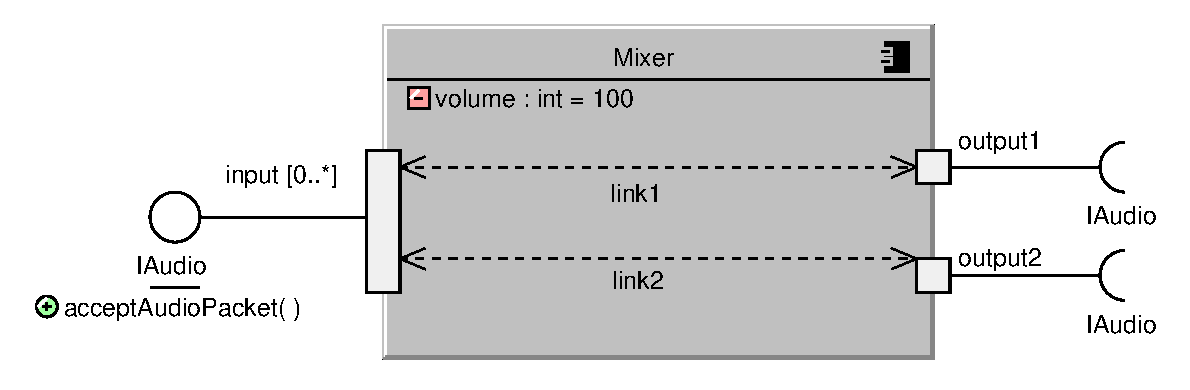
\includegraphics[scale=0.5]{model-images/mixer-leaf}
\par\end{centering}

\caption{\label{fig:The-mixer-leaf}The mixer leaf component}

\end{figure}


The mixer is a leaf component, which means that is cannot be decomposed
further into other component instances. Each leaf must be directly
associated with a Java implementation class which implements the logic.
The volume is held as an attribute, which is set to a default value.

Instead of defining a device component at this point, we will define
a placeholder (figure \ref{fig:A-placeholder-device}). This is a
dummy (composite) component which outlines the general shape that
any device should have. A placeholder can be used to indicate something
that must be concretely defined later, and is intended to be descriptive
rather than prescriptive.

%
\begin{figure}
\begin{centering}
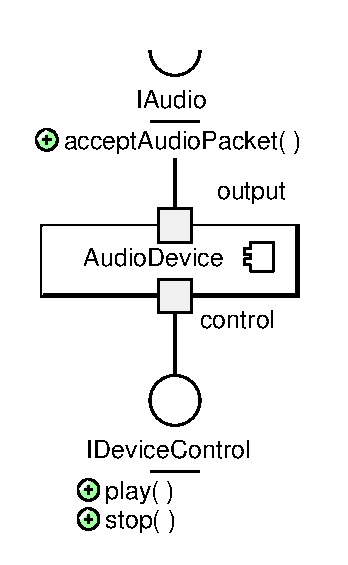
\includegraphics[scale=0.5]{model-images/device-placeholder}
\par\end{centering}

\caption{\label{fig:A-placeholder-device}A placeholder device shows the {}``shape''
of an audio device}

\end{figure}


We can now define the desk component (figure \ref{fig:The-desk-composite}).
The desk is a composite component, consisting of an instance of the
mixer component and an instance of the device placeholder. These instances
are also known as \emph{parts}. They are wired together using connectors,
which connect ports.

A desk contains a mixer, and exposes its outputs. It contains devices
which are connected between the indexed \emph{input} and \emph{deviceControl}
ports. The latter is how the desk is controlled.

%
\begin{figure}[h]
\begin{centering}
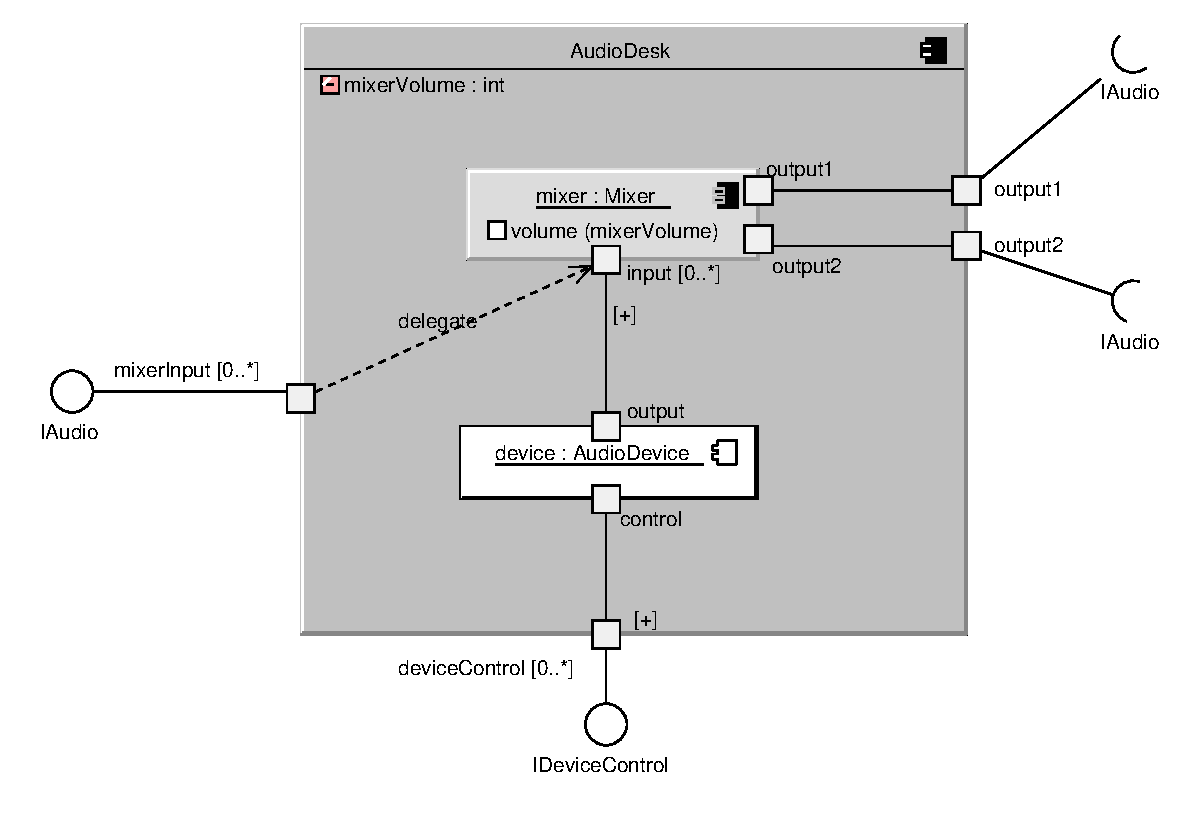
\includegraphics[scale=0.5]{model-images/desk-composite}
\par\end{centering}

\caption{\label{fig:The-desk-composite}The desk composite has a mixer and
a device part}

\end{figure}


It is worth noting that the desk component cannot be instantiated
as it contains a placeholder. This must be replaced, through resemblance
or redefinition, before use.

The \emph{{[}+]} (pronounced {}``take next'') is used to connect
to an indexed port, and will assign the next available index to the
connector. In this case, the assigned index will be zero. The use
of \emph{{[}+]} prevents connectors from independently independent
extensions from taking the same index.

A delegate connector is used to connect the \emph{mixerInput} and
\emph{input} ports. This aliases two ports together, and is used to
prevent the need for many indexed connectors between two indexed ports.


\subsection{\label{sub:Port-Type-Inference}Port Type Inference}

The function of port type inference is to automatically infer the
interfaces of a port in a composite component. This minimises the
changes required when later modifying components using resemblance
or redefinition.

The port links (\emph{link1}, \emph{link2}) in the leaf mixer component
are used to propagate port type information if {}``more is provided
than is required''. For instance, if an instance of mixer is connected
so that a sub-interface of IAudio is provided to both \emph{output1}
and \emph{output2} then this will result in \emph{input} also providing
the sub-interface -- the type information has propagated via the links.
This also works the other way -- if input was connected to something
that required the sub-interface, then this would propagate through
so that the outputs also required that sub-interface. Port links reflect
the internal connections of a leaf, as leaves have no explicit connectors.

The interfaces required and provided by a port (the port's type) of
a composite component can always be inferred. Whilst this is a trivial
matter in the case of figure \ref{fig:The-desk-composite}, the inference
rules are useful when replacing parts of a component using the constructs
provided for extension. The changes will automatically propagate such
that the port types update also.

Composites cannot explicitly specify port links: the links for a composite
can always be inferred from the connections between the component
and the parts. To support an incremental approach, the port type inference
algorithm will determine a set of inferred links for each composite,
which indicate how any internal parts propagate type information between
ports. The inferred links for the desk are shown in figure \ref{fig:The-inferred-links}.
This shows that the \emph{mixerInput} and \emph{output1} and \emph{output2}
ports are linked, reflecting the links from the mixer part that they
connect via.

%
\begin{figure}
\begin{centering}
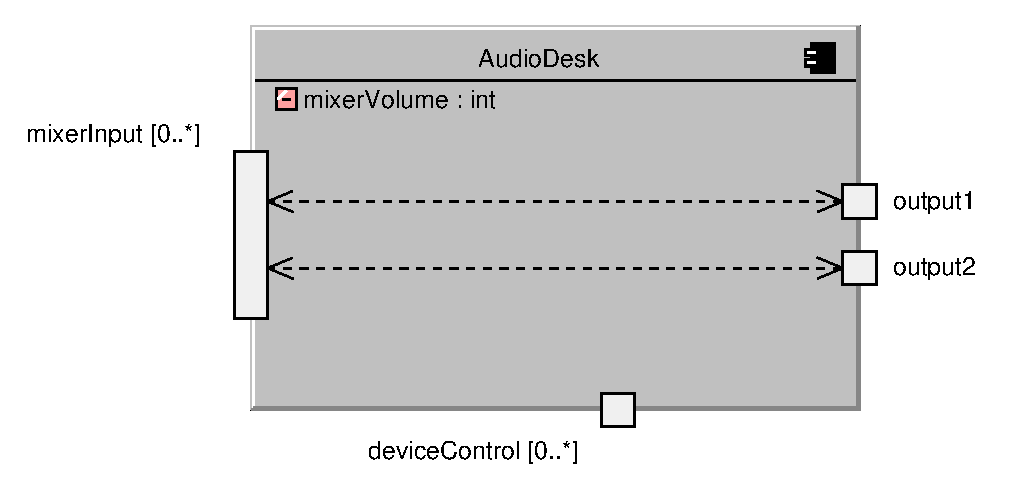
\includegraphics[scale=0.5]{model-images/inferred-links}
\par\end{centering}

\caption{\label{fig:The-inferred-links}The inferred links of the desk component}

\end{figure}



\subsection{Slots and Aliasing}

The mixer defines a volume attribute. An attribute is of primitive
type (int, boolean etc) and provides a view on the internal configuration
state of a component. An attribute may have a default value, such
as in figure \ref{fig:The-mixer-leaf}.

When we create a part, we can assign values to each of the attributes
of the part's type. These are known as slots. When a slot has a value
assigned, there are three possibilities:

\begin{enumerate}
\item A literal assignment.\\
E.g. volume = 100. This will initialise the attribute with the literal
value.
\item A copy assignment from the environment.\\
E.g. volume = mixerVolume. This will copy the value of the attribute
over from the parent component, but the attribute values can then
diverge.
\item An attribute alias.\\
E.g. volume(mixerVolume). This aliases the part attribute with an
attribute from the parent component.
\end{enumerate}
For the mixer part in figure \ref{fig:The-desk-composite}, the third
option is used which binds the two attributes together into a single
one. \emph{This allows us to propagate state from one or more parts
into the parent component.} This has allowed us to encapsulate the
mixer in the desk, but still allow the mixer's volume to be configured
at the desk level.


\subsection{Packaging the Application}

We now have our base application. To package it into a single entity,
we use a stratum which is a module-like construct based around the
UML2 package concept. A stratum contains component and interface definitions.
A stratum may not contain other strata, for reasons of simplicity
rather than any technical necessity.

Each stratum must explicitly express its dependencies on other strata.
These dependencies constrain the elements that are visible to the
stratum's elements. In the case of our application there are no dependencies,
as we package everything into a single stratum called Desk (figure
\ref{fig:The-desk-stratum}).

%
\begin{figure}
\begin{centering}
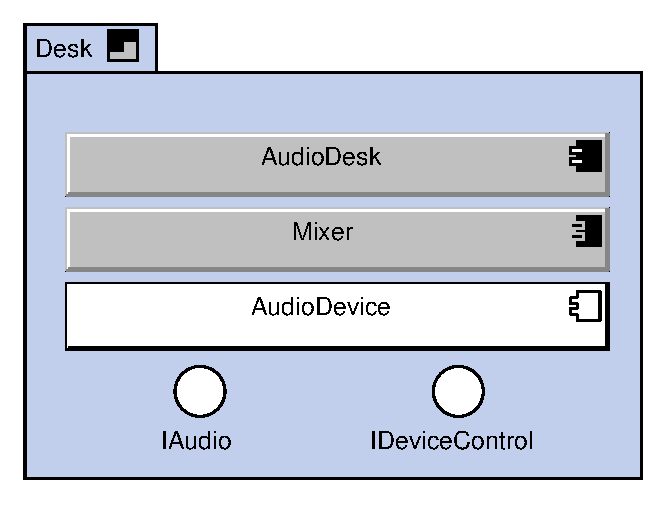
\includegraphics[scale=0.5]{model-images/desk-stratum}
\par\end{centering}

\caption{\label{fig:The-desk-stratum}The desk stratum packages the application
into a single entity}

\end{figure}



\subsection{Summary}

Backbone's architectural approach is similar to that provided by Darwin
\cite{Magee1995}. It is based on the UML2 composite structure model
\cite{OMGUML}. Strata are not entirely dissimilar to modules, which
serve to group elements in an application. The reasons for the existence
of both strata and components are similar to the ones outlined for
the coexistence of modules and classes in \cite{Bruce1998}.

A hierarchy of components can be created through composition. This
focus on hierarchy, composition and encapsulation allows large architectures
to be defined, managed and reasoned about at the appropriate level
of abstraction (MANAGE). This is one of the key aspects that differentiates
Backbone over conventional plugin architectures \cite{Object2001}.

Backbone describes a composite component as a connected configuration
of other component instances (parts). This captures more of the architecture
than an object-oriented description of a system where the instantiations
are contained within code. Further, the requirement that a component
express both provided and required interfaces enforces a disciplined
approach to dependencies. It is often the case when using an object
oriented approach that classes have many code-defined dependencies
on definitions of other classes, leading many to a complex and implicit
tangle of dependencies \cite{Foote1999}.

Port type inference allows the interfaces provided and required by
ports in a composite component to be inferred. As well as saving time,
this features limits the changes required when altering parts of the
application in order to extend it. Port links provide a way to propagate
type information through the ports of a leaf, and are used to represent
the internal connections. This is necessary because leaves do not
have explicit connectors. This allows leaf components to be more reusable,
as will be shown when the mixer is able to automatically adjust for
a sub-interface of IAudio (section \ref{sub:Port-Type-Inference}).


\section{Extending the Application: Adding a CD Player}

An independent developer, X, is asked by a radio station to extend
the desk so that it can operate a CD player device. X must use the
application as provided by AudioSoft.

The controller for the CD player device is shown in figure \ref{fig:The-CD-player}.
Note that it does not conform exactly to the shape of the device placeholder
component, as it provides an additional interface (IDeviceCue).

%
\begin{figure}
\begin{centering}
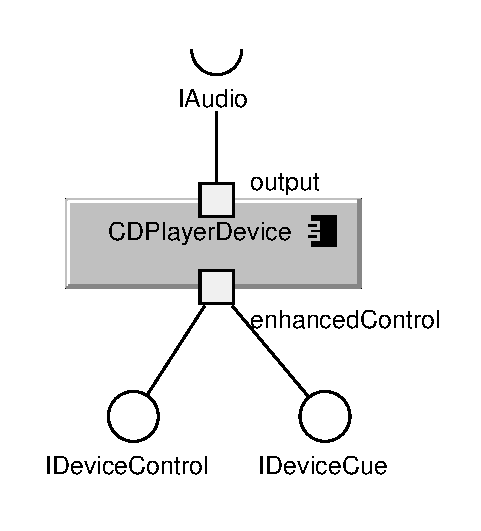
\includegraphics[scale=0.5]{model-images/cd-player}
\par\end{centering}

\caption{\label{fig:The-CD-player}The CD player component}

\end{figure}



\subsection{Resemblance}

The developer decides to make an AudioDeskWithCD component which is
similar to AudioDesk, but adds a CD player. To define this, the \emph{resemblance}
construct is used, which allows a new component to be defined in terms
of delta changes to one or more existing components. Figure \ref{fig:Defining-a-new}
shows the graphical view of the new component, along with the textual
view underneath.

%
\begin{figure}[h]
\begin{centering}
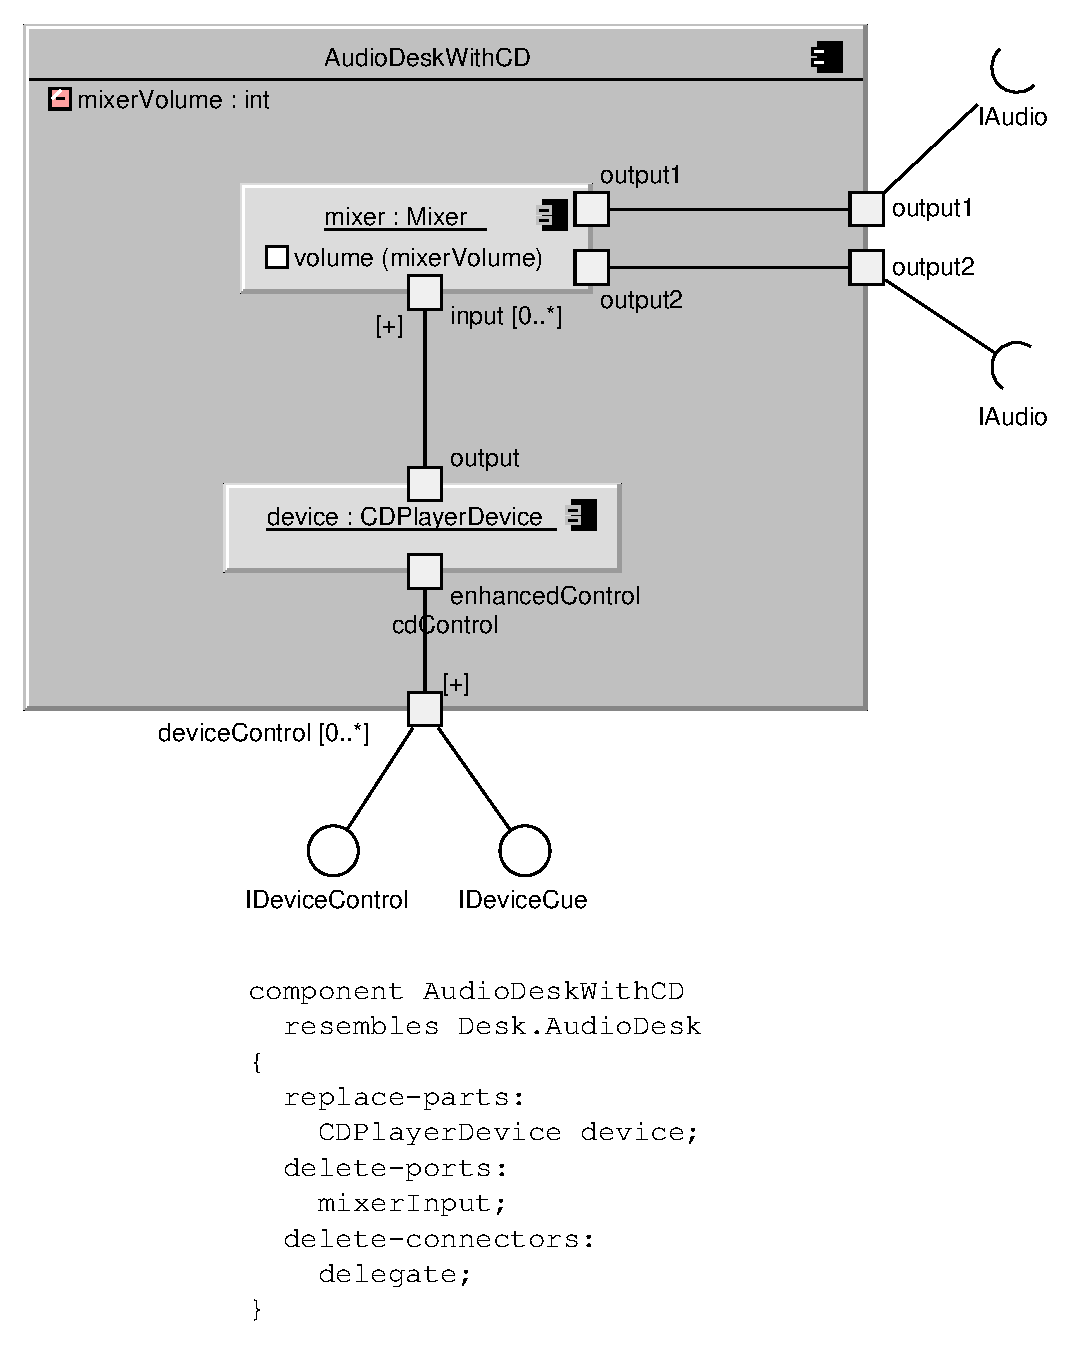
\includegraphics[scale=0.5]{model-images/audiodesk-with-cd}
\par\end{centering}

\caption{\label{fig:Defining-a-new}Defining a new desk component in terms
of differences to the original one}

\end{figure}


The placeholder device has been replaced by a CD player part, and
the \emph{mixerInput} port and \emph{delegate} connector have been
removed because they were not required by developer X. Port type inferencing
has determined that the \emph{deviceControl} port now provides both
IDeviceControl and IDeviceCue.

Note that this is a distinct component from AudioDesk. However, since
the new component is defined in terms of changes, if AudioDesk changes,
then the new component will change also. This feature allows us to
accept upgraded (UPGRADE) versions of AudioDesk in the future, possibly
defined using redefinition (section \ref{sub:Redefinition}).


\subsection{Packaging the Extension}

The two components are packaged in the DeskWithCD stratum. The components
depend on definitions in the Desk stratum, and so we must explicitly
indicate this using a dependency (figure \ref{fig:The-DeskWithCD-stratum}).
Another way to look at it is that the strata level dependencies constrain
what the elements in a stratum can refer to. With the dependencies
as shown, the elements in DeskWithCD can only refer to elements in
that stratum, or the Desk stratum.

%
\begin{figure}[h]
\begin{centering}
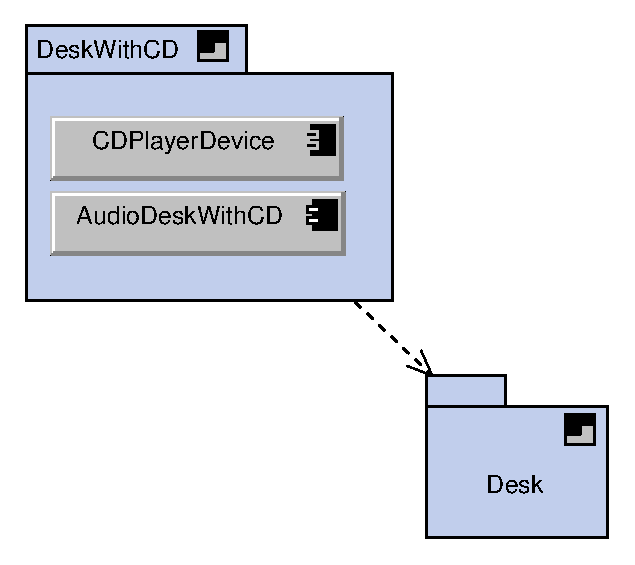
\includegraphics[scale=0.5]{model-images/desk-extension-packaging}
\par\end{centering}

\caption{\label{fig:The-DeskWithCD-stratum}The DeskWithCD stratum depends
on the Desk stratum}

\end{figure}



\subsection{\label{sub:Wrap}Summary}

Using resemblance to define a new component in terms of another has
several advantages over a completely new definition. It is economical
and convenient -- only the changes need be specified. In addition,
if the resembled component changes at some point or is upgraded, then
so does the new component's definition (UPGRADE).

For a composite component, changes can be addition, replacement or
deletion or ports, parts, connectors and attributes. This gives the
extension developer a large amount of flexibility to remodel the {}``insides''
that it has inherited (EXTEND). This is in contrast to object-oriented
inheritance where only additions and explicit overrides (limited replacement)
can be performed \cite{Taivalsaari1996}.

Multiple resemblance is allowed, as long as the resemblance graph
is acyclic (see section \ref{sec:Rules}).

Resemblance is not allowed for leaf components. This sidesteps the
troublesome issue of a composite resembling a leaf and vice versa.
To get around this restriction, in an actual system, leaf components
are wrapped immediately in an {}``identity'' composite, which is
then used instead of the leaf (E.g. figure \ref{fig:Leaves-are-always}).
The composite wrapper can then be redefined or resembled. The intention
is to have this wrapping managed automatically by the graphical CASE
tool supporting the Backbone approach, freeing the designer from this
burden \cite{McVeigh2006}.

%
\begin{figure}[h]
\begin{centering}
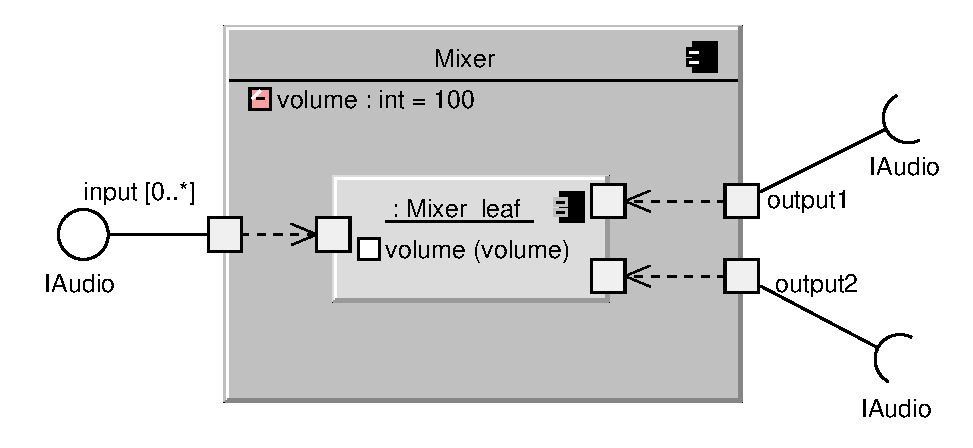
\includegraphics[scale=0.5]{model-images/wrapped-mixer}
\par\end{centering}

\caption{\label{fig:Leaves-are-always}Leaves are always wrapped by {}``identity
composites'' in reality}

\end{figure}


Packaging a set of definitions as a stratum provides a useful, coarse-grained
view of the dependency structure of a large application. Strata dependencies
cannot be cyclic, and this focuses the developer on maintaining a
strict layering of the architecture. A stratum can be understood in
terms of its own elements and those of the strata that it depends
upon. A single stratum can contain an arbitrary number of component
and interface definitions, and an extension is usually packaged as
a single stratum that depends on the strata defining the application
that it is extending.


\section{Evolving the Application: Adding a Microphone}

AudioSoft decides to evolve the desk application to version 1.1, adding
a microphone device as standard. AudioSoft has no knowledge of developer
X or the changes made to support the CD player.

The microphone component is shown in figure \ref{fig:The-microphone-leaf}.
Of particular interest is that it requires the IExtendedAudio interface
rather than just the IAudio interface. This is because the microphone
must continually monitor the output (via getMaximumLevel) to ensure
that its output does not exceed the maximum level.

%
\begin{figure}[h]
\begin{centering}
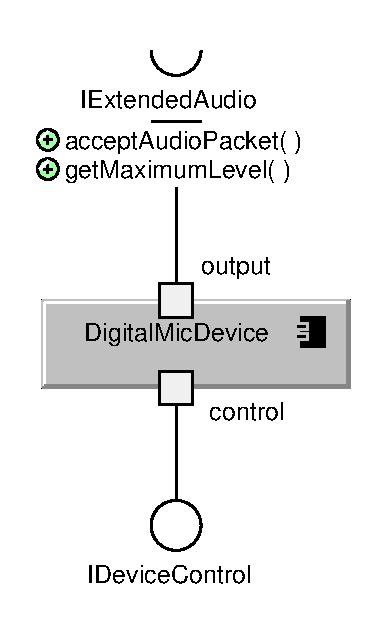
\includegraphics[scale=0.5]{model-images/mic}
\par\end{centering}

\caption{\label{fig:The-microphone-leaf}The microphone leaf component}

\end{figure}



\subsection{Interface Resemblance}

Figure \ref{fig:Resembling-an-interface} shows that IExtendedAudio
is defined in terms of resemblance from IAudio. In this case, we have
added a single operation (getMaximumLevel) and hence IExtendedAudio
is a sub-interface of IAudio. It is also possible to delete and replace
operations in the resembling definition, but doing this will break
the subtype relation.

Inheritance is not used in Backbone. This concept has been subsumed
by resemblance, which allows deletion and arbitrary replacement in
addition to addition and overriding.

%
\begin{figure}[h]
\begin{centering}
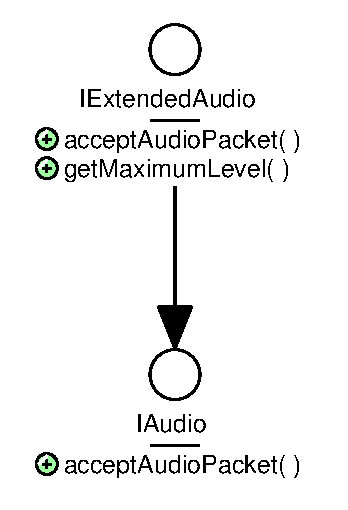
\includegraphics[scale=0.5]{model-images/extended-audio}
\par\end{centering}

\caption{\label{fig:Resembling-an-interface}Resembling an interface and adding
operations preserves the subtype relation}

\end{figure}


Interfaces and composite components can redefine and resemble elements
of the same type. Multiple resemblance is supported in both cases
as long as the resemblance graph is acyclic at all times.


\subsection{\label{sub:Redefinition}Redefinition}

Because they are evolving the platform, Audiosoft must change the
desk component. However, they do not wish to force existing users
of the previous version to upgrade. \emph{Redefinition} can be used
to support this.

Redefinition allows a new component definition to be substituted for
an existing one. The reason for using redefinition in this case is
that AudioDesk is being evolved. Simply producing a new component
definition with a microphone in it would mean that every product using
the existing desk component would need to be upgraded.

In this case, resemblance and redefinition are used together to evolve
the AudioDesk component to include a new device (figure \ref{fig:Redefining-the-desk}).
The microphone and two connectors have been added, and the original
placeholder kept.

%
\begin{figure}[h]
\begin{centering}
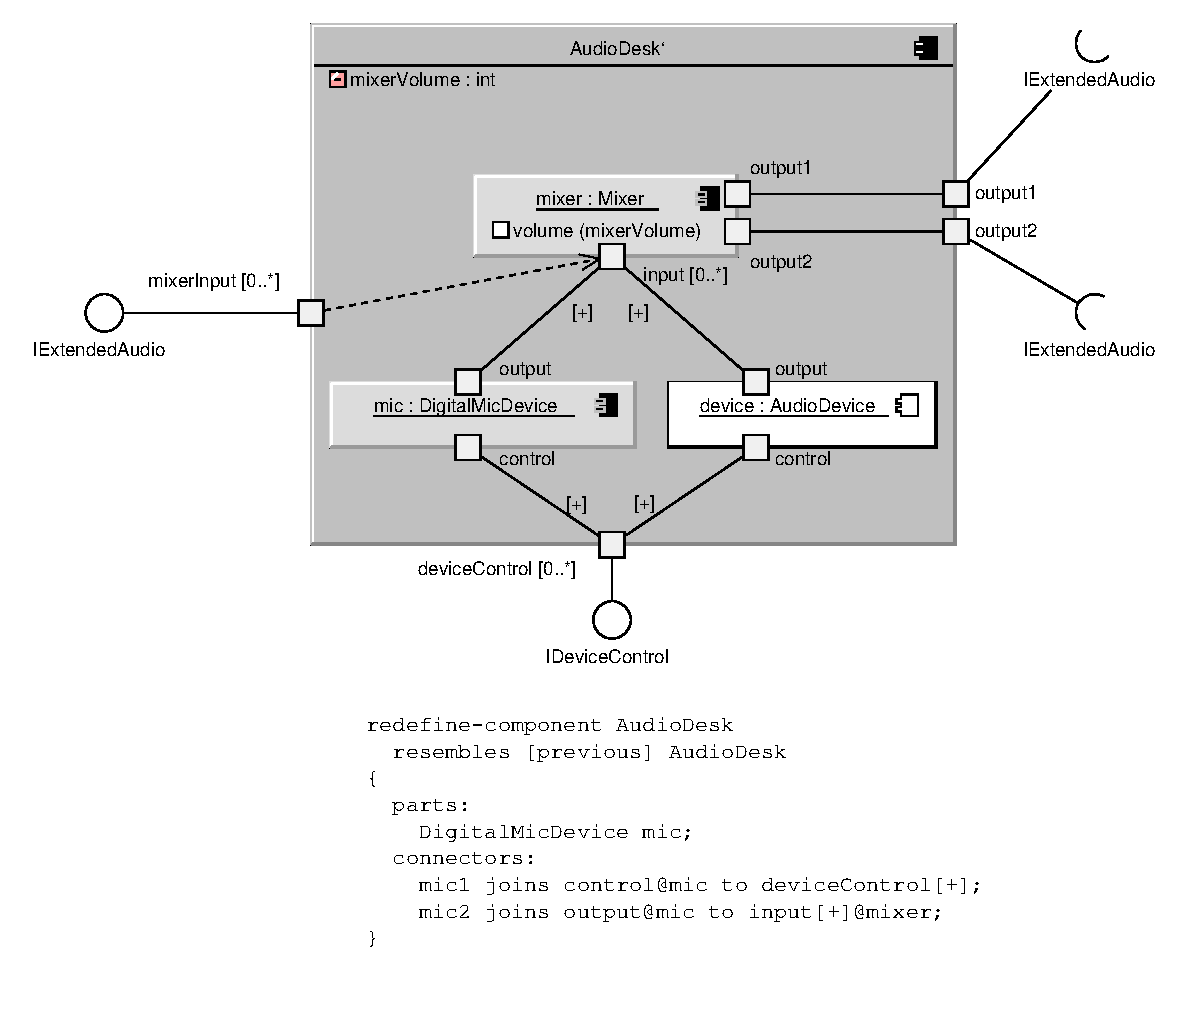
\includegraphics[scale=0.5]{model-images/redefined-desk}
\par\end{centering}

\caption{\label{fig:Redefining-the-desk}Redefining the desk component to add
a microphone.}

\end{figure}


It is important to note that the definition of \emph{mixerInput},
\emph{output1} and \emph{output2} have automatically been upgraded
by the port type inferencing rules. Because the output port of DigitalMicDevice
requires IExtendedAudio, then this requirement propagates through
the port links to ensure that \emph{output1} and \emph{output2} now
require the sub-interface.

Similarly, the mixer \emph{input} port must now provide IExtendedAudio.
This is also exposed outside of the component via the \emph{mixerInput}
port.

The redefinition succeeded with only three additions because IExtendedAudio
is a sub-interface of IAudio. It is possible for the mixer \emph{input}
port to provide IExtendedAudio, which satisfies both the microphone
and placeholder device. If it were not a sub-interface, then it would
still be possible to add the microphone, but it would require the
mixer and device components to also be redefined to ensure compatibility
with the new interface.


\subsection{Packaging the Extension}

The extension is packaged in the EvolvedDesk (version 1.1) stratum,
as shown in figure \ref{fig:Packaging-the-evolved}. To allow the
evolved definitions to reference the original definitions in the Desk
stratum, a dependency must be present between the two strata.

%
\begin{figure}[h]
\begin{centering}
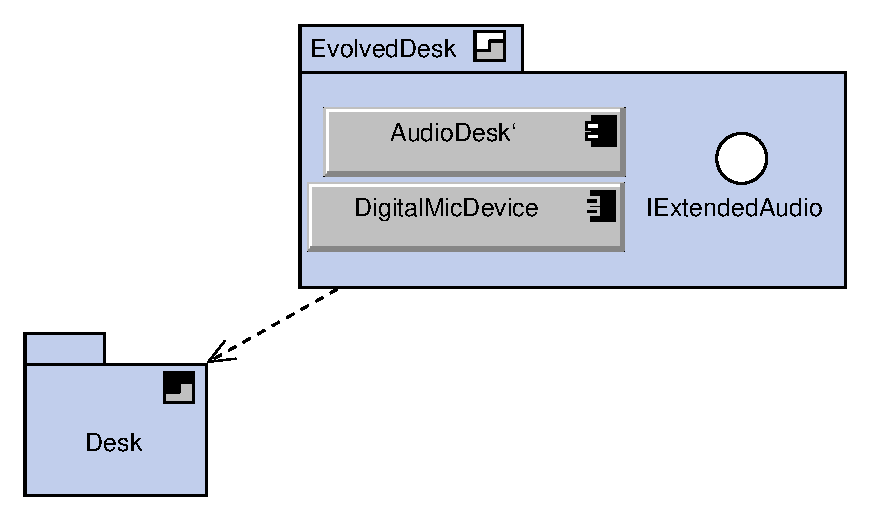
\includegraphics[scale=0.5]{model-images/evolved-desk-packaging}
\par\end{centering}

\caption{\label{fig:Packaging-the-evolved}Packaging the evolved desk in a
stratum}

\end{figure}


The EvolvedDesk stratum has a slightly different icon, indicating
that it is \emph{relaxed} rather than \emph{strict}. A relaxed stratum
will propagate its dependencies to any stratum which further depends
on it. In effect, it allows other stratum to {}``see through it''
to the stratum that it depends on. This can be used to support \emph{strict}
and \emph{relaxed} styles of application layering, or a combination
of the two \cite{Buschmann1996}.


\subsection{The Overlapping Extensions Problem}

The Backbone interpreter must be provided with a list of included
strata in order to assemble a system. If we provide it with only the
Desk stratum, then the AudioDesk component will be as defined in figure
\ref{fig:The-desk-composite}. If however, we provide it with the
EvolvedDesk and Desk strata, then the AudioDesk component will be
defined as in figure \ref{fig:Redefining-the-desk}.

This is called stratum perspective. The desk from the perspective
of the Desk stratum is the original definition (figure \ref{fig:The-desk-composite}).
From the perspective of EvolvedDesk, it is the redefined definition
(figure \ref{fig:Redefining-the-desk}). The \emph{home stratum} of
a component is the stratum in which it is defined.

The EvolvedDesk and DeskWithCD strata do not depend on each other.
X has developed the CD player extension directly against desk rather
than the evolved version. The way that the dependencies are defined,
no element from DeskWithCD can refer to anything introduced in EvolvedDesk
and vice versa. The two strata are said to be \emph{mutually independent}
(section \ref{sub:Definition-of-Terms}), and the dependencies imply
that the strata were developed independently (without knowledge of
each other).

However, both strata share a common dependency in the Desk stratum.
The two strata are said to \emph{overlap}. Mutually independent, overlapping
strata are used to model architectural extensions which have been
developed independently.

It is the case that mutually independent strata that overlap can cause
conflicts when combined. This is because each stratum can make adjustments
to the underlying overlapped strata that will conflict when used together.
We call this potential for conflict the \emph{overlapping extensions}
\emph{problem}.


\subsection{\label{sub:Port-Type-Inference}Port Type Inference Revisited: Top
Down Development}

The port type inferencing (section \ref{sub:Port-Type-Inference})
of Backbone works in concert with the redefinition and resemblance
constructs. When the microphone was added in this case, the \emph{mixerInput},
\emph{output1} and \emph{output2} ports were all automatically adjusted
to cope with the sub-interface that was required.

This works well with bottom-up development where a composite is defined
after its constituent parts have already been defined. In this case,
the port types can be determined using inference. However, this causes
a problem for top-down development where the decomposition of a composite
is not yet available.

To support top-down development, the interfaces provided and required
by a port may be explicitly specified for a composite (they must always
be specified for a leaf). These will be checked against the inferred
port interfaces for the home stratum of the component, where they
must be the same if the component is considered to be well-formed.
However, from the perspective of other stratum, only the inferred
port interfaces are used (if available). In our example, it was possible
to explicitly define the desk's \emph{mixerInput} port as providing
IAudio if this was desired. However, from the perspective of EvolvedDesk,
the port provides IExtendedAudio because of the port type inferencing
rules. The original, explicity indicated port type is ignored outside
of its home stratum.

Placeholders can also be used to support top down development \cite{Medvidovic1996a}.


\subsection{Summary}

Backbone provides the redefinition construct for representing the
evolution of a component. This confers a similar level of flexibility
to the extension developer as is already available to the application
developer (EXTEND). Redefinition allows a component in an underlying
stratum to be replaced with a new definition. When combined with resemblance,
redefinition allows a component to be incrementally evolved. A component
can only redefine one other, which is not in the same stratum. Note
that a redefinition cannot be directly referred to -- we must instead
refer to the component being redefined.

A redefinition does not affect the underlying application unless its
owning stratum is explicitly included in the graph that the Backbone
interpreter sees. The original application developers do not need
to see the changes, or adjust their application to accommodate them
(NO\_IMPACT). This also allows the extension developer freedom to
add new features that the base application developers would not normally
consider.

In this example, AudioSoft has used redefinition to evolve an application,
keeping the changes due to evolution separate from the original application.
Users of the original application are not affected, but can choose
to upgrade by combining their extensions with the evolving extension.

Backbone does not limit the changes that can be made to an application
and can model the arbitrary evolution of components. However, it is
in the developer's best interest to keep the changes small, in order
to minimise the chance of conflicts between overlapping but mutually
independent extensions. As will be shown later in this chapter, any
conflicts can be resolved using redefinition.


\section{Combining Extensions: Adding a Microphone and a CD Player}

Unsurprisingly, another developer Z wishes to have a desk with both
a CD player and a microphone. Z decides to use both extensions DeskWithCD
and EvolvedDesk together . As the two stratum are independently developed
and overlapping, structural and behavioural conflicts are possible
when we try to use both at the same time. These conflicts are due
to the different modifications and assumptions that the independent
developers made when adapting the base application.


\subsection{Combining Two Overlapping Extensions}

All that is necessary to merge a number of overlapping strata is to
create a further stratum that depends on them. If the Backbone interpreter
is then given this stratum, it will construct a system based on this
perspective.

For the example, we define the UnifiedDesk stratum to combine DeskWithCD
and EvolvedDesk (figure \ref{fig:Combining-two-overlapping}).

%
\begin{figure}[h]
\begin{centering}
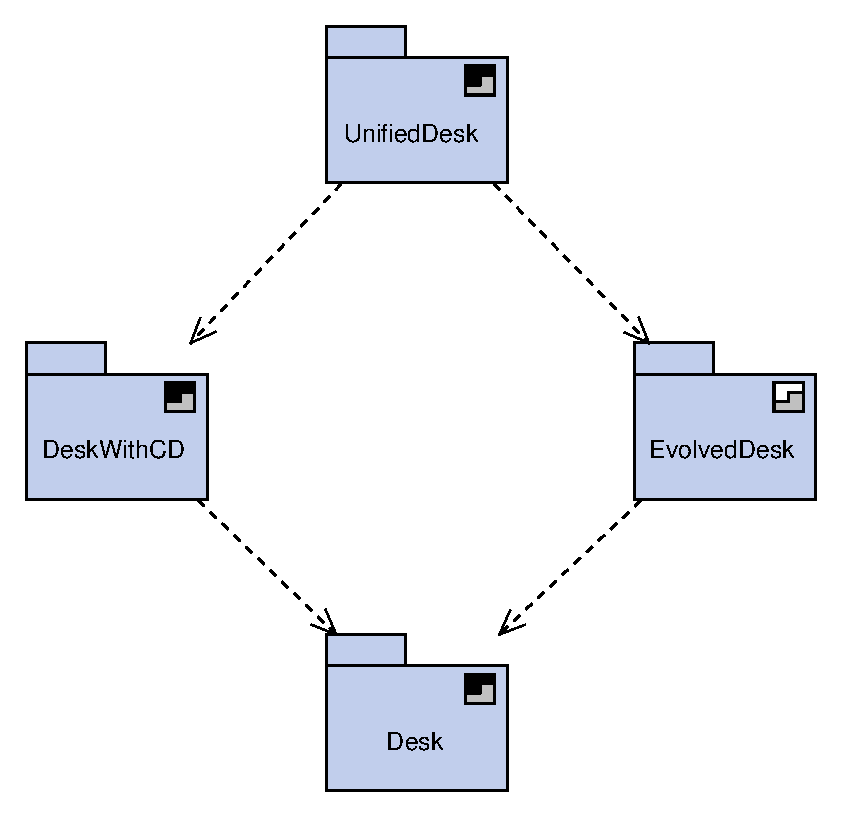
\includegraphics[scale=0.5]{model-images/unified}
\par\end{centering}

\caption{\label{fig:Combining-two-overlapping}Combining two overlapping extensions}

\end{figure}



\subsection{Redefinition Is Rewritten as Resemblance}

Redefinition is handled by rewriting the resemblance graph of each
component to take any redefinitions into account (section \ref{sub:Element-Rules}).
All resemblance graphs are recalculated for each stratum perspective.
Figure \ref{fig:Redefinition-is-rewritten} shows the resemblance
graph of AudioDeskWithCD from the perspective of UnifiedDesk. The
topmost element of the graph becomes the AudioDeskWithCD component.

%
\begin{figure}[h]
\begin{centering}
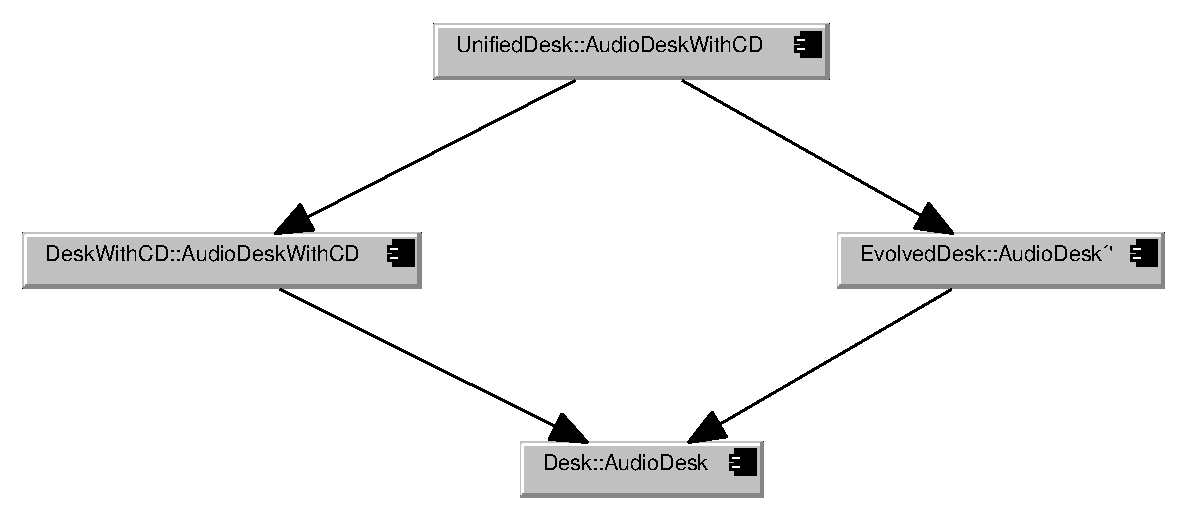
\includegraphics[scale=0.5]{model-images/redefinition-rewritten}
\par\end{centering}

\caption{\label{fig:Redefinition-is-rewritten}Redefinition is rewritten into
the resemblance graph}

\end{figure}


Conflicts may occur because changes made in different branches of
the resemblance graph conflict in some way. This is not the only way
that conflict occurs. Another possibility is that a redefinition in
one overlapping extension is incompatible with a definition in another
independently developed extension causing a well-formedness rule to
be violated. In practice, conflicts can be subtle.

From the perspective of UnifiedDesk, the AudioDesk component is the
same as the redefinition shown in figure \ref{fig:Redefining-the-desk}.
There are no conflicting redefinitions to this component that must
be reconciled. However, the redefinition has changed the definition
of the desk component that AudioDeskWithCD resembles, thereby also
changing the definition of AudioDeskWithCD.

The UnifiedDesk::AudioDeskWithCD component is implicitly created by
the Backbone system in order to form a complete graph. The expanded
structure of this component is shown in figure \ref{fig:The-conflicted-AudioDeskWithCD}.
The deletion of mixerInput has been applied as requested by AudioDeskWithCD,
and both devices are present. However, there is no possible definition
of the \emph{deviceControl} port that can satisfy both the microphone
(IDeviceControl) and the CD player (IDeviceControl and IDeviceCue)
and the component is marked as malformed. We have a structural conflict
that requires developer intervention.

%
\begin{figure}[h]
\begin{centering}
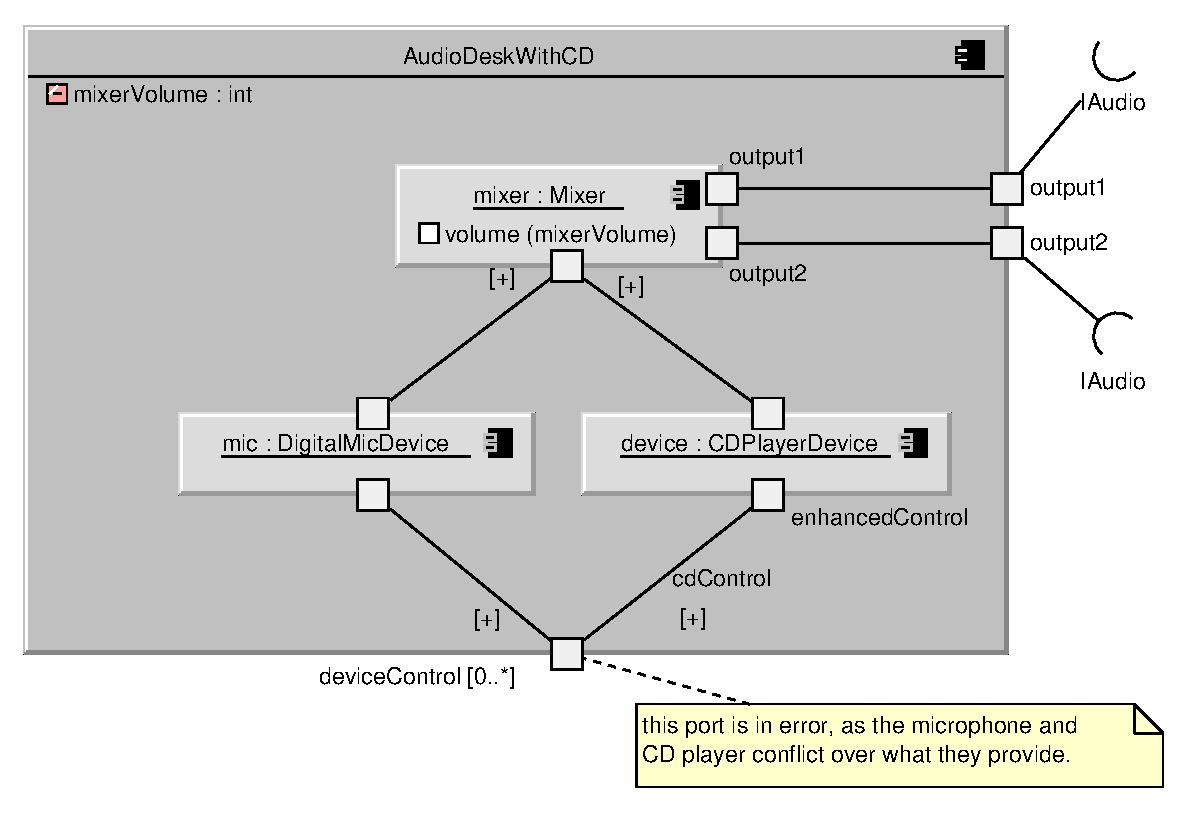
\includegraphics[scale=0.5]{model-images/conflicted-audiocd}
\par\end{centering}

\caption{\label{fig:The-conflicted-AudioDeskWithCD}The conflicted AudioDeskWithCD
component}

\end{figure}


Using a redefinition we can resolve the conflict neatly as shown in
figure \ref{fig:Resolving-the-conflict}. A further port named \emph{extendedControl}
is created which provides both device and cue control. The CD player's
control port is routed to this new port.

%
\begin{figure}[h]
\begin{centering}
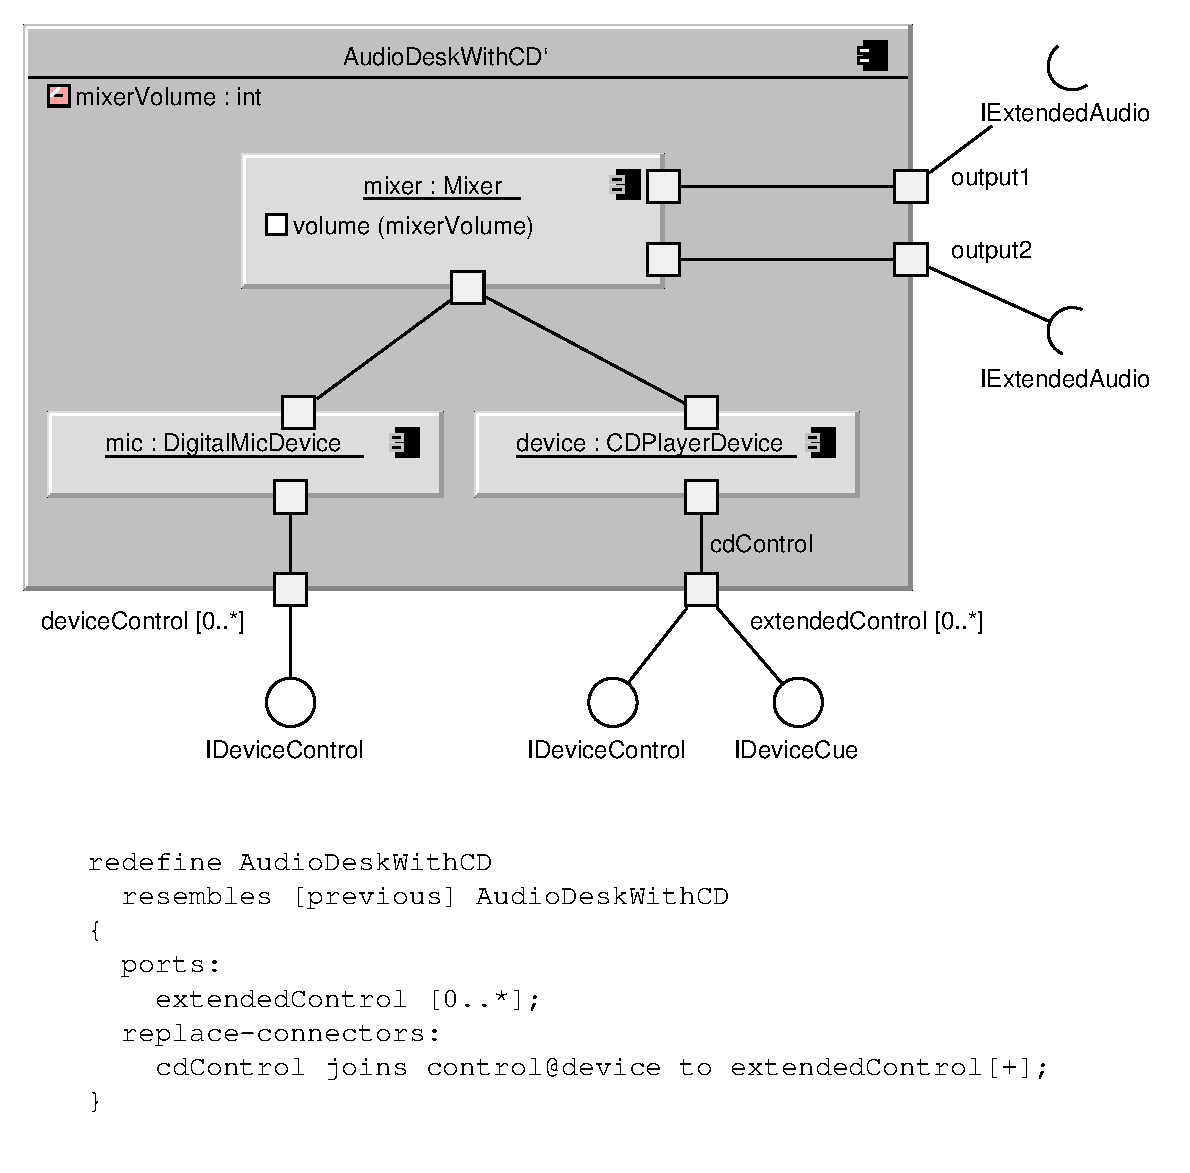
\includegraphics[scale=0.5]{model-images/resolved-audiocd}
\par\end{centering}

\caption{\label{fig:Resolving-the-conflict}Resolving the conflict by creating
another port}

\end{figure}



\subsection{Summary}

Conflicts can occur when mutually independent and overlapping extensions
are combined. Combination is possible because changes are kept as
deltas (COMBINE). Conflict can always be resolved by further redefinitions,
which make the developer's intentions explicit (VERIFY\_AND\_REPAIR).
The key is to keep the number of changes as small as possible so that
the chance of further conflict with other extensions is minimised.
Well-formedness rules pick up structural conflict (VERIFY\_AND\_REPAIR).

Redefinition is rewritten into each component's resemblance graph,
for each stratum perspective. Multiple resemblance can occur when
combining overlapping extensions, as the rewritten graph must take
into account the partial strata order. The detection and resolution
of conflicts does not rely on a total order being specified for strata,
unlike other approaches \cite{Ichisugi2002}.


\section{Dynamic Instantiation: Adding Feed Devices}

The configurations presented so far have been static. Component instantiation
occurs at start-up time, when the interpreter creates the required
parts for the given configuration. However, in most applications a
level of dynamic instantiation is required. To support this, Backbone
provides \emph{isomorphic factory} components. These are composite
components which lazily instantiate their parts on demand, and can
instantiate multiple times. As composites, they can be redefined and
resembled. They are isomorphic because the structure of the factory
mimics the structure of the lazily created parts and connectors.

Consider that a developer wishes to add a number of audio feed devices
to the desk. There are up to ten feeds available, each requiring a
separate controller, and we wish to create these devices on demand.
The definition of AudioFeedDevice is shown in figure \ref{fig:An-audio-feed}.

%
\begin{figure}[h]
\begin{centering}
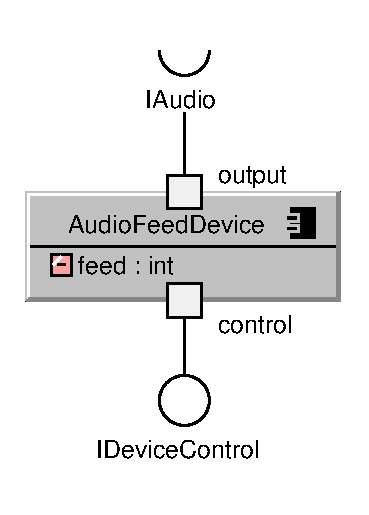
\includegraphics[scale=0.5]{model-images/feed-device}
\par\end{centering}

\caption{\label{fig:An-audio-feed}An audio feed device controls audio from
feed inputs}

\end{figure}


In order to instantiate feed devices lazily, a factory must be created
(figure \ref{fig:A-factory-for}). This is similar to a normal composite,
except that it contains a create port which is not attached internally.
The Backbone interpreter will locate this port and provide an internal
implementation with the correct factory behaviour. The port will also
contain functionality allowing the configuration attributes of the
factory to be set (setFeed).

%
\begin{figure}[h]
\begin{centering}
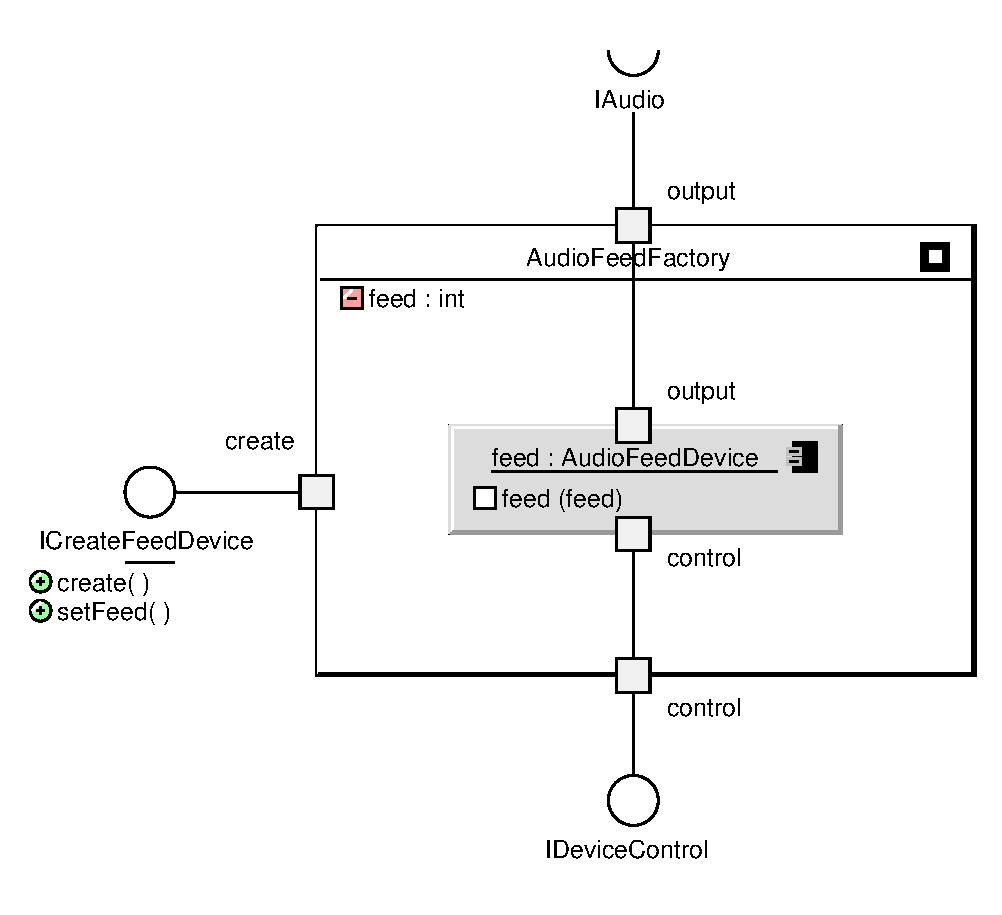
\includegraphics[scale=0.5]{model-images/audio-feed-factory}
\par\end{centering}

\caption{\label{fig:A-factory-for}A factory for instantiating audio feed devices}

\end{figure}


Finally, to configure this into the desk, we create a new component
AudioDeskWithFeeds which resembles AudioDesk (figure \ref{fig:Wiring-up-the}).
The factory's create port has been exposed on the outside of the desk,
and can be used to instantiate feeds. It is necessary to explicitly
set the feed attribute via the create port before instantiating another
part. Note that \emph{{[}+]} is used on the connections from the factory
so that a different index will be used each time.

%
\begin{figure}[h]
\begin{centering}
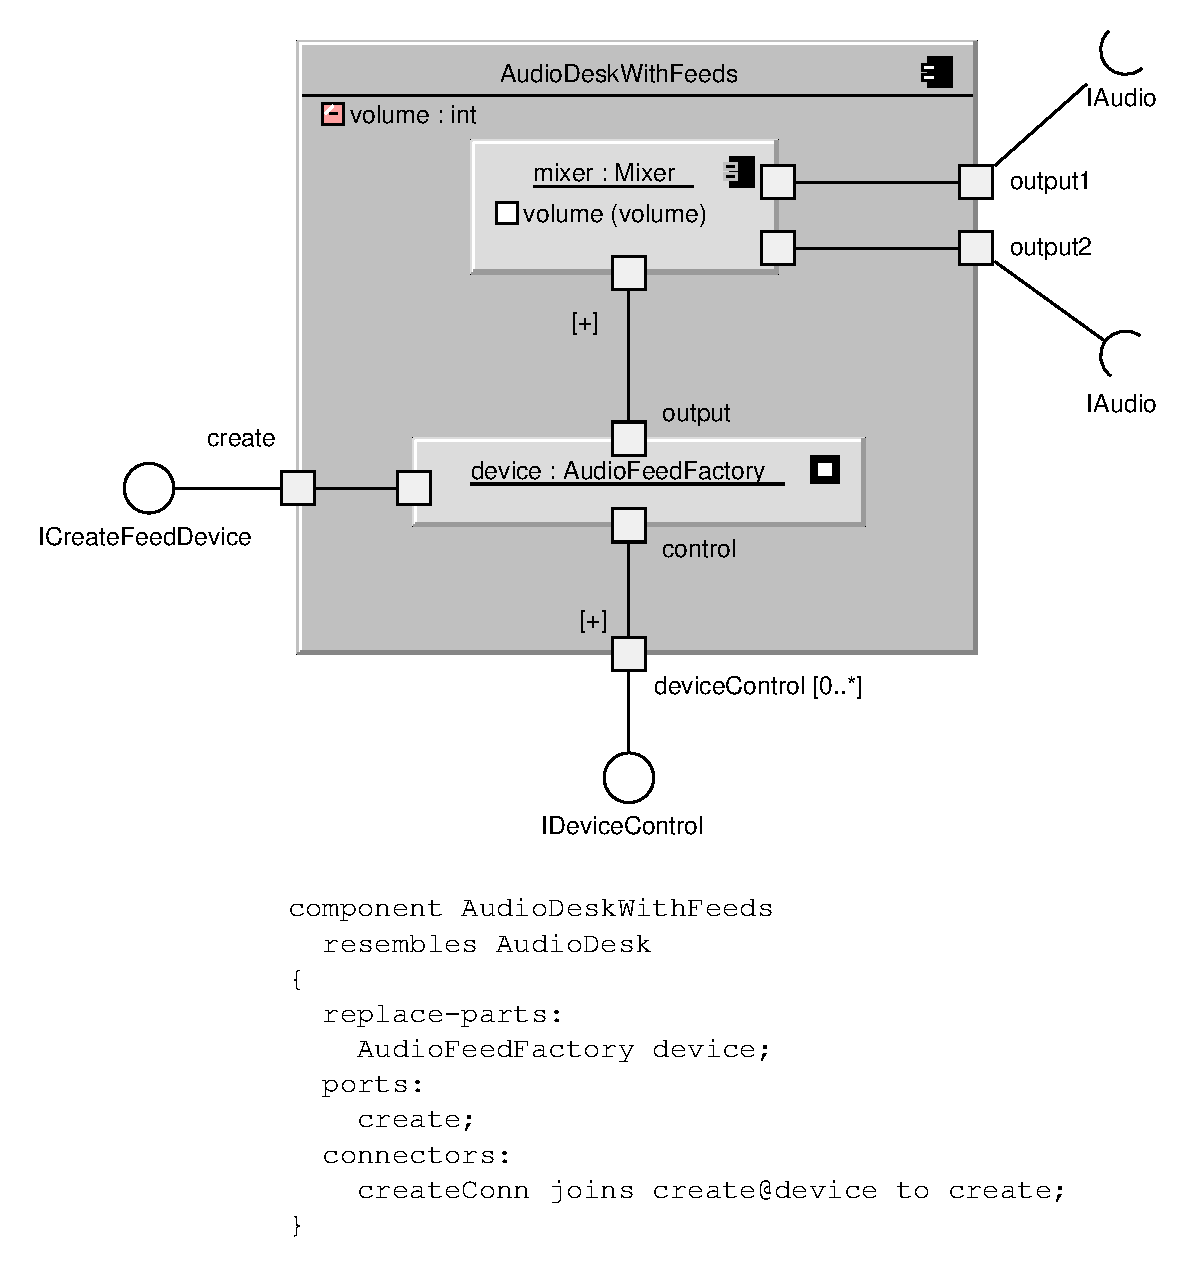
\includegraphics[scale=0.5]{model-images/audiodesk-with-feeds}
\par\end{centering}

\caption{\label{fig:Wiring-up-the}Wiring up the feed factory into a desk component}

\end{figure}



\subsection{Summary}

Dynamic component instantiation is supported by factory components.
As these are composite components, they can be redefined, resembled
and may contain placeholders. This allows a number of useful architectural
techniques to be used, including creating a factory which acts as
a base component for a set of factories which resemble it. The \emph{{[}+]}
construct helps with multiple instantiation, allowing separate instantiations
to take different indices.


\section{Summary: Backbone as an Extension Architecture}

The Backbone approach is designed to support creating and managing
architectures and extending them. Extension developers have the freedom
to make arbitrary changes to the underlying application, and the constructs
support the division of concerns between extension and application
developers. The hierarchical model simplifies the definition and management
of the complex application architectures (MANAGE). By allowing an
extension to adjust the architecture at the appropriate level, change
is kept to a minimum which also minimises the chances of any conflicts
between independently developed, overlapping extensions.

The changes are specified to the architectural definition, not to
the implementation code. This allows the approach to work even when
the implementation code is not available, as long as the Backbone
architectural description of the system is given. This partially addresses
the requirement not to reveal source code in the EXTEND requirement.

Resemblance allows one component to be defined in terms of delta changes
to another. Redefinition allows a new definition to be substituted
for an existing component, and models component evolution. Redefinition
and resemblance together allow existing components to be incrementally
modified by an extension (EXTEND). Port type inference cuts down the
number of changes required when adding or removing parts from existing
components (UPGRADE).

Note that the resembling and redefining components are kept in delta
form, and applied to the original definitions at application start-up
time. The use of deltas makes possible the combination of extensions,
and subsequent repair of conflicts.

Overlapping extensions can be combined using a further extension which
brings them together via strata dependencies. This allows multiple
redefinitions to be combined into a unified system (COMBINE). Structural
conflicts are picked up by well-formedness rules, and can be resolved
using further redefinitions (VERIFY\_AND\_REPAIR).

The Backbone approach is also applicable for component reuse and integration,
given that the requirements for dealing with application extensibility
represent a superset of these requirements. The constructs provided
reduce the abstraction problem, which results from trying to reuse
highly specific components which encode assumptions deep within their
composition hierarchy \cite{Greenfield2004}. Redefinition and reuse
can be used to alter such components to fit into a new context \cite{McVeigh2006}.


\subsection{Limitations}

The approach has some limitations in practice:

\begin{itemize}
\item Cross-cutting concerns are not handled well.\\
Like conventional component-based systems, cross-cutting concerns
such as logging and security must be handled in the traditional manner
where logic may be spread across many components. Also, changing an
interface may have a wide-ranging impact on the definition of a system.
Redefinition can always handle the required {}``repairs'', but these
may be extensive and may cut through many component definitions. Port
type inference helps by propagating type changes, but this cannot
handle the implementation implications of deleting an operation of
an interface, for example.
\item Modeling with deltas is sometimes inconvenient.\\
It is not always convenient to model changes uniformly using the constructs
provided. For some types of change, it is often simpler just to modify
the application directly. In circumstances where this type of modification
is permissible or even possible, Backbone provides support for checking
that the changes are compatible with existing extensions.
\item Dynamic extension is not supported.\\
The Backbone runtime model does not support the dynamic application
of extensions. This reflects a limitation of the runtime interpreter,
rather than a fundamental issue with the approach.
\item The application must be specified using Backbone.\\
In order to take advantage of the extensibility constructs, an application
must be specified in Backbone. To retrofit the Backbone approach onto
an existing object-oriented application can involve significant changes
and refactoring.
\end{itemize}
%
\begin{comment}
\bibliographystyle{plain}
\bibliography{\string"/home/amcveigh/work/workspace/Academic Work/read papers/references\string"}

\end{comment}
{}
\end{document}
